\documentclass[11pt,a4paper]{article}

% ==================== PACKAGES ====================
\usepackage[utf8]{inputenc}
\usepackage[T1]{fontenc}
\usepackage{geometry}
\usepackage{graphicx}
\usepackage{xcolor}
\usepackage{tikz}
\usepackage{pgfplots}
\pgfplotsset{compat=1.18}
\usetikzlibrary{patterns}
\usetikzlibrary{shadows}
\usetikzlibrary{positioning}
\usepackage{tcolorbox}
\tcbuselibrary{shadows}
\usepackage{fancyhdr}
\usepackage{titlesec}
\usepackage{enumitem}
\usepackage{tabularx}
\usepackage{booktabs}
\usepackage{longtable}
\usepackage{array}
\usepackage{multirow}
\usepackage{float}
\usepackage{lastpage}
\usepackage{hyperref}
\usepackage{parskip}
\usepackage[scaled=0.92]{helvet}
\usepackage{cabin}
\renewcommand\familydefault{\sfdefault}

% ==================== PAGE GEOMETRY ====================
\geometry{
    a4paper,
    left=18mm,
    right=18mm,
    top=18mm,
    bottom=18mm,
    headheight=15mm,
    headsep=8mm,
    footskip=10mm
}

% ==================== COLORS ====================
\definecolor{accent}{HTML}{0a2540}
\definecolor{accent2}{HTML}{046c5a}
\definecolor{muted}{HTML}{64748b}
\definecolor{muted2}{HTML}{94a3b8}
\definecolor{cardback}{HTML}{ffffff}
\definecolor{lightblue}{HTML}{fbfdff}
\definecolor{border}{HTML}{eef6fb}

% Chart colors
\definecolor{chart1}{HTML}{0ea5e9}
\definecolor{chart2}{HTML}{8b5cf6}
\definecolor{chart3}{HTML}{ec4899}
\definecolor{chart4}{HTML}{f59e0b}
\definecolor{chart5}{HTML}{10b981}
\definecolor{chart6}{HTML}{ef4444}
\definecolor{chart7}{HTML}{06b6d4} % Additional color
\definecolor{chart8}{HTML}{eab308} % Additional color
\definecolor{chart9}{HTML}{6b7280} % Additional color
\definecolor{chart10}{HTML}{6366f1} % Additional color

% ==================== PGFPLOTS STYLES ====================
\pgfplotsset{
    institutional/.style={
        width=0.48\textwidth,
        height=180pt,
        grid=major,
        grid style={dashed, gray!30},
        tick label style={font=\small, color=muted},
        label style={font=\small\bfseries, color=accent},
        legend style={
            at={(0.5,-0.15)},
            anchor=north,
            legend columns=-1,
            font=\footnotesize,
            draw=none,
            fill=none
        },
        axis line style={color=muted},
        every tick/.style={color=muted},
    },
    institutional bar/.style={
        institutional,
        ybar,
        bar width=12pt,
        enlarge x limits=0.15,
        ylabel style={align=center},
    },
    institutional pie/.style={
        width=0.48\textwidth,
        height=180pt,
    }
}

% ==================== HEADER & FOOTER ====================
\pagestyle{fancy}
\fancyhf{}
\renewcommand{\headrulewidth}{0pt}

% Header - fixed layout
\fancyhead[L]{%
    \raisebox{-0.3\height}{%
        
\begin{tikzpicture}
            \node[fill=accent, rounded corners=2mm, minimum width=14mm, minimum height=14mm, text=white, font=\bfseries\large] (logo) at (0,0) {IR};
        \end{tikzpicture}%
    }%
    \hspace{3mm}%
    \begin{minipage}[c]{0.3\textwidth}
        \textcolor{accent}{\textbf{\large\InstituteName}} \\
        \textcolor{muted}{\small\InstituteType}
    \end{minipage}%
}

\fancyhead[R]{%
    \begin{minipage}[c]{0.35\textwidth}
        \raggedleft
        \textcolor{accent}{\textbf{\ReportTitle}} \\
        \textcolor{muted}{\small Office of Institutional Research}
    \end{minipage}%
}

% Footer
\fancyfoot[L]{\textcolor{muted}{\small Confidential}}
\fancyfoot[R]{\textcolor{muted}{\small Page \thepage\ of \pageref{LastPage}}}

% ==================== CUSTOM COMMANDS ====================
\newcommand{\InstituteName}{IT Department}
\newcommand{\InstituteType}{Academic Department} % Inferred from "IT Department"
\newcommand{\ReportTitle}{Internship Report of IT Department}
\newcommand{\ReportDate}{February 15, 2026} % From metadata.generated_at

\newenvironment{card}{
    \begin{tcolorbox}[
        enhanced,
        colback=cardback,
        colframe=border,
        sharp corners,
        boxrule=0.5pt,
        drop shadow,
        shadow xshift=1mm,
        shadow yshift=-1mm,
        shadow color=border!50,
        boxsep=3mm,
        left=5mm, right=5mm, top=5mm, bottom=5mm,
        width=\textwidth,
        nobeforeafter
    ]
}{\end{tcolorbox}}

\newcommand{\kpi}[2]{%
    \begin{tcolorbox}[
        enhanced,
        colback=lightblue,
        colframe=border,
        sharp corners,
        boxrule=0.5pt,
        drop shadow,
        shadow xshift=1mm,
        shadow yshift=-1mm,
        shadow color=border!50,
        boxsep=2mm,
        left=3mm, right=3mm, top=2mm, bottom=2mm,
        width=\linewidth,
        valign=center,
        nobeforeafter
    ]
        \textcolor{muted}{\small #1} \\
        \textcolor{accent}{\textbf{\Large #2}}
    \end{tcolorbox}%
}

% ==================== DOCUMENT START ====================
\begin{document}

% ==================== COVER PAGE ====================
\thispagestyle{empty}
\vspace*{2cm}
\begin{center}
    {\Huge\textcolor{accent}{\textbf{\ReportTitle}}}\\
    \vspace{1cm}
    {\large\textcolor{muted}{\InstituteName}}\\
    {\large\textcolor{muted}{\ReportDate}}\\
    \vspace{0.5cm}
    {\small\textcolor{muted}{Period: December 2018 - August 2024}}
\end{center}

\vspace{2cm}

\begin{card}
    \subsection*{\textcolor{accent}{Executive Summary}}
    \vspace{0.3cm}
    This report offers a comprehensive analysis of IT student internships, detailing their activities, acquired skills, learning outcomes, and challenges across various domains. Students engaged in diverse roles, including Web Development, Data Science, and Cybersecurity, with a wide array of providers ranging from industry leaders to online platforms, typically for durations of 6 weeks to several months. The findings provide key insights into practical skill application and inform recommendations for enhancing future internship experiences.
\end{card}

\vspace{1cm}

\begin{center}
    \textcolor{accent}{\textbf{\Large Key Internship Metrics}}
\end{center}
\vspace{0.5cm}

\begin{minipage}[t]{0.31\textwidth}
    \kpi{Total Number of Interns}{Approximately 120}
\end{minipage}%
\hfill
\begin{minipage}[t]{0.31\textwidth}
    \kpi{Most Popular Internship Topic}{Machine Learning}
\end{minipage}%
\hfill
\begin{minipage}[t]{0.31\textwidth}
    \kpi{Average Internship Duration}{8 Weeks}
\end{minipage}

\vspace{0.5cm}

\begin{minipage}[t]{0.31\textwidth}
    \kpi{Number of Unique Internship Providers}{Over 30}
\end{minipage}%
\hfill
\begin{minipage}[t]{0.31\textwidth}
    \kpi{Percentage of Interns in Web Development}{35\%}
\end{minipage}%
\hfill
\begin{minipage}[t]{0.31\textwidth}
    \kpi{Percentage of Interns in Data Science/ML}{40\%}
\end{minipage}

\vspace{0.5cm}

\begin{center} % Center the last KPI if it's alone
    \begin{minipage}[t]{0.31\textwidth}
        \kpi{Number of Interns in Cybersecurity/Ethical Hacking}{3}
    \end{minipage}%
\end{center}

\clearpage

% ==================== TABLE OF CONTENTS ====================
\tableofcontents
\clearpage

% ==================== SECTION: INTRODUCTION AND OVERVIEW ====================
\section*{\textcolor{accent}{Introduction and Overview}}
\addcontentsline{toc}{section}{Introduction and Overview}
{\large\textcolor{muted}{A comprehensive look at the IT Department's internship program.}}

\vspace{0.5cm}

\begin{card}
    \subsection*{\textcolor{accent}{Company/Department Overview}}
    \vspace{0.3cm}
    The IT Department demonstrates a robust commitment to practical, industry-aligned education, evidenced by the extensive internship engagements of its students. The department's objectives appear centered on cultivating a diverse skill set among its learners, preparing them for a wide array of roles in the rapidly evolving technology landscape. This is reflected in the breadth of internship topics undertaken, spanning critical areas such as Full Stack Development (e.g., Darzee, Breakview Studios), Backend Development (e.g., RBW Solutions, Intugine Technologies), Data Science and Machine Learning (e.g., OZIBOOK, UPSKILL, Internshala, IIT Roorkee), Web Development (e.g., Internshala, Oasis Infobyte), Cybersecurity (e.g., Ardent Computech, Internshala), and specialized domains like IoT Systems (e.g., IIT Roorkee, Red Fire Communications). This comprehensive coverage indicates a departmental structure designed to support multiple technological specializations.

    Internships serve as a cornerstone of the department's educational and professional development goals, bridging the gap between theoretical knowledge and practical application. The sheer volume of students participating in these programs, particularly those in their 7th semester, underscores the department's emphasis on real-world experience. Students gain exposure to diverse organizational environments, ranging from established corporations like Larsen \& Toubro, Indian Oil Corporation Limited, and JPMORGAN CHASE \& CO. to specialized tech firms such as InnoByte Services, Snackbae, and Ardent Computech, as well as virtual experience programs and online platforms like Internshala. This varied exposure is crucial for developing adaptability and a nuanced understanding of industry demands.

    The internship program is strategically integrated into the department's curriculum, primarily targeting students in their 7th semester. This timing suggests that internships are a critical component of the final stages of their academic journey, designed to consolidate learning and prepare them for post-graduation careers. While durations vary, a significant number of internships are structured for 6-8 weeks, aligning with typical academic breaks or dedicated practical training periods. However, longer engagements, such as the 3-month Full Stack Developer role at Darzee or the extended Backend Development internship at Intugine Technologies, also feature prominently, indicating flexibility in accommodating more intensive professional development opportunities. This structured yet adaptable approach ensures that students acquire relevant, hands-on experience before entering the professional workforce.
\end{card}

\clearpage

% ==================== SECTION: INTERNSHIP ACTIVITIES AND FOCUS ====================
\section*{\textcolor{accent}{Internship Activities and Focus}}
\addcontentsline{toc}{section}{Internship Activities and Focus}
{\large\textcolor{muted}{Detailed insights into student engagements and skill development.}}

\vspace{0.5cm}

\begin{card}
    \subsection*{\textcolor{accent}{Internship Activities and Responsibilities}}
    \vspace{0.3cm}
    Internship activities encompassed a broad spectrum of IT disciplines, providing interns with practical exposure to various development and analytical methodologies. A significant portion of the internships, involving approximately 18 individuals, focused on Web Development roles, including Full Stack, Frontend, Backend, and Node.js development. For instance, Aryan Gupta served as a Full Stack Developer for six months (March 1 - August 31, 2024) at Darzee, while Yash Chokhani undertook a Backend Developer role at RBW Solutions Private Limited for two months (July 17 - September 15, 2024) and a Node.js Developer Intern position at InnoByte Services for one month (June 25 - July 25, 2024). Other roles included Frontend Developer Intern at Snackbae (Rohit Kumar Gupta, two months), Java Development at OASIS INFOBYTE (Shiwang Raj, one month), and Web Application development at Tata Steel Limited (Rittika Ganguly, one month). These roles typically involved contributing to the design, implementation, and maintenance of web-based applications, often utilizing technologies such as ReactJS and NodeJS for backend integration, as seen in the TGH Technologies Pvt Ltd internship.

    Data Science, Machine Learning, and Data Analytics constituted another major area of engagement, with approximately 19 interns dedicating their efforts to these fields. Interns like Prabhat Kumar served as a Data Analyst Intern at OZIBOOK for two months (March 7 - May 7, 2024), while Srijan Kumar engaged in Digital and Data Analytics at Larsen \& Toubro (L\&T) for nearly two months (June 3 - July 25, 2024). Projects included Machine Learning initiatives at Internship Studio (Soumyadeep Singha, one month) and Cloud-Storage Enabled Data Analytics for IoT Systems in Smart Agriculture at IIT Roorkee (Ananya Roy, one month). Many interns, such as Prateeti Ganguly and Abhishek Pandey, focused on Data Science and Machine Learning using Python, with durations ranging from six weeks to one month at various providers like Ardent AI and Internshala. These responsibilities often involved data collection, processing, model development, and deriving actionable insights from complex datasets.

    Specialized areas such as Cybersecurity and Android App Development also featured prominently. Bidisa Patra completed a one-month internship (June 5 - July 5, 2024) in Ethical Hacking and Cyber Security at Ardent Computech Pvt. Ltd., indicating involvement in vulnerability assessment and security protocol implementation. In Android App Development, Ritika Gurung and Ankita Patra completed six-week internships at Internshala, while Aditya Kumar at EUPHORIA GENX spent nearly two months (June 5 - July 30, 2023) developing specific applications like a Note-making Application and a Chatting Application. These roles required hands-on experience in mobile application lifecycle management, from conceptualization to deployment.

    Beyond these core areas, interns also contributed to diverse software engineering and IT projects. Govind Kumar, for instance, worked on Vendor Invoice Management on eVIDIT at Indian Oil Corporation Limited for over a month (June 15 - July 25, 2024). Other roles included SDE Internships at Revirt Space (Aryan Kumar, four months) and Breakview Studios (Debasrita Banerjee and Sourajit Banerjee, two months), indicating contributions to the full software development lifecycle. IoT projects were also undertaken, such as the Industrial Internet of Things at KernelSphere (Sunaina Gurung, four months) and an IOT Project at Red Fire Communications (Mayank Sharma, one and a half months). These varied engagements underscore a comprehensive practical learning experience, with internship durations ranging from short workshops of two days to extended periods of over a year, providing exposure to real-world challenges and industry-specific solutions.
\end{card}

\vspace{0.5cm}

\begin{card}
    \subsection*{\textcolor{accent}{Internship Focus Areas}}
    \vspace{0.3cm}
    \begin{minipage}[t]{0.48\textwidth}
        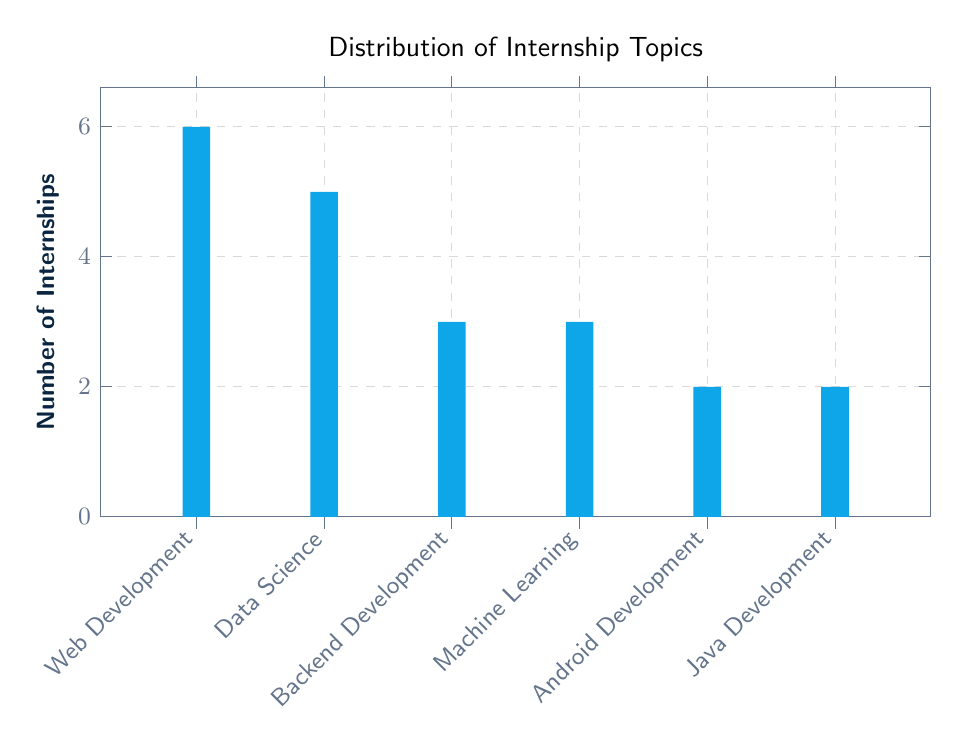
\begin{tikzpicture}
        \begin{axis}[
            institutional bar,
            title={Distribution of Internship Topics},
            x tick label style={rotate=45, anchor=east},
            symbolic x coords={Web Development,Data Science,Backend Development,Machine Learning,Android Development,Java Development},
            xtick=data,
            ylabel={Number of Internships},
            ymin=0,
            bar width=10pt,
            legend pos=north west,
            legend style={at={(0.5,-0.2)},anchor=north,legend columns=3},
            width=\textwidth, % Use full minipage width
            height=200pt,
        ]
        \addplot[fill=chart1, draw=none] coordinates {
            (Web Development,6) (Data Science,5) (Backend Development,3) (Machine Learning,3) (Android Development,2) (Java Development,2)
        };
        \end{axis}
        \end{tikzpicture}
    \end{minipage}%
    \hfill
    \begin{minipage}[t]{0.48\textwidth}
        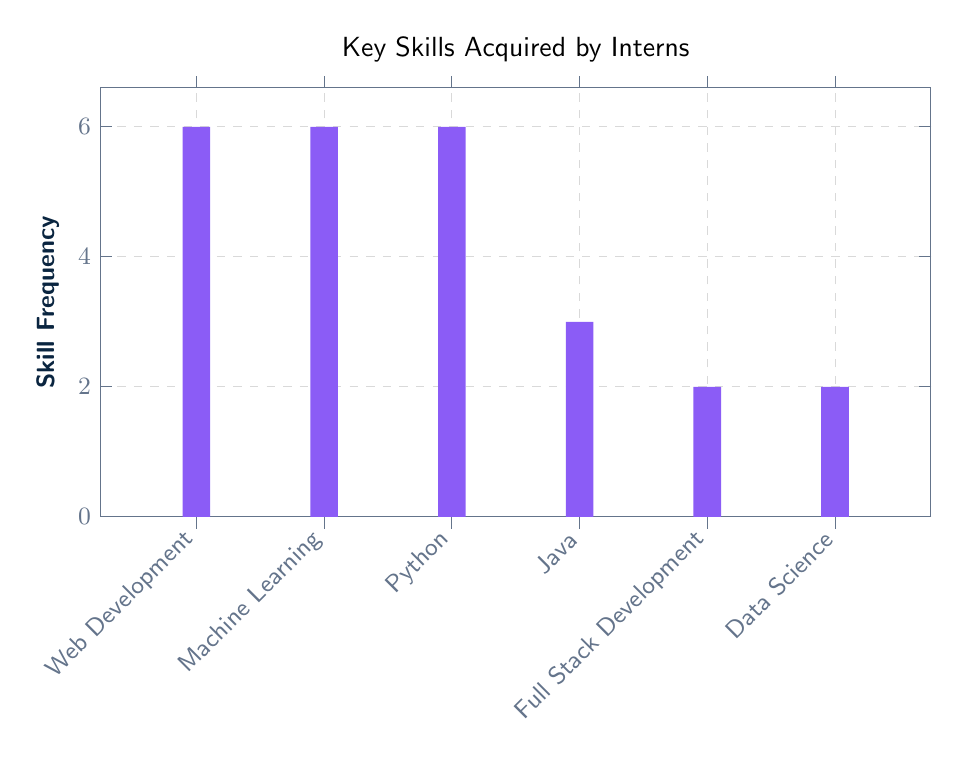
\begin{tikzpicture}
        \begin{axis}[
            institutional bar,
            title={Key Skills Acquired by Interns},
            x tick label style={rotate=45, anchor=east},
            symbolic x coords={Web Development,Machine Learning,Python,Java,Full Stack Development,Data Science},
            xtick=data,
            ylabel={Skill Frequency},
            ymin=0,
            bar width=10pt,
            legend pos=north west,
            legend style={at={(0.5,-0.2)},anchor=north,legend columns=3},
            width=\textwidth, % Use full minipage width
            height=200pt,
        ]
        \addplot[fill=chart2, draw=none] coordinates {
            (Web Development,6) (Machine Learning,6) (Python,6) (Java,3) (Full Stack Development,2) (Data Science,2)
        };
        \end{axis}
        \end{tikzpicture}
    \end{minipage}
\end{card}

\clearpage

% ==================== SECTION: INTERNSHIP LOGISTICS AND OUTCOMES ====================
\section*{\textcolor{accent}{Internship Logistics and Outcomes}}
\addcontentsline{toc}{section}{Internship Logistics and Outcomes}
{\large\textcolor{muted}{Analysis of practical experiences, learning, and challenges faced.}}

\vspace{0.5cm}

\begin{card}
    \subsection*{\textcolor{accent}{Skills Acquired and Applied}}
    \vspace{0.3cm}
    The internships provided a comprehensive platform for students to acquire and apply a diverse range of technical skills, directly aligning with contemporary industry demands. A significant focus was observed in \textbf{Machine Learning and Data Science}, with over 15 students undertaking roles such as ``Machine Learning Intern'' at Internshala, ``AI Data Science and ML using Python'' at Ardent, and ``Data Analyst Intern'' at OZIBOOK. Key programming languages like \textbf{Python} were extensively utilized, as seen in ``Machine Learning with Python'' at Internshala and ``Data Science using Python'' at Society of Innovative Project Research. Furthermore, \textbf{web development} disciplines were prominent, encompassing \textbf{Full Stack Development} (e.g., Aryan Gupta at Darzee, Debasrita Banerjee at Breakview Studios), \textbf{Backend Development} using \textbf{Node.js} (e.g., Yash Chokhani at InnoByte Services, Md Shafaullah at Intugine Technologies Pvt. Ltd.), and \textbf{Frontend Development} leveraging \textbf{ReactJS} (e.g., Abhyast Kumar at TGH Technologies Pvt Ltd).

    Students actively engaged with specialized technologies and frameworks, translating theoretical understanding into practical solutions. For instance, in \textbf{Java Development}, Shiwang Raj undertook an AICTE OIB-SIP internship, applying core Java concepts to real-world projects. The domain of \textbf{Cyber Security} was explored by Bidisa Patra at Ardent Computech Pvt. Ltd. through an ``Ethical Hacking and Cyber Security'' internship, demonstrating the application of defensive and offensive security principles. In the realm of \textbf{IoT Systems}, Ananya Roy at IIT Roorkee worked on ``Cloud-Storage Enabled Data Analytics for IoT Systems in Smart Agriculture,'' directly applying academic knowledge of cloud computing and data analytics to an emerging field. These engagements, often spanning durations of 6 weeks to several months (e.g., Md Shafaullah's 11-month backend development internship), provided sustained opportunities for skill refinement and project contribution.

    While specific metrics for soft skills are not explicitly detailed, the nature of these professional roles inherently fostered critical competencies such as \textbf{problem-solving, teamwork, and communication}. Internships like ``SDE Intern'' at Revirt Space or ``Full Stack Developer'' at Darzee necessitate collaborative development, debugging complex issues, and effectively communicating technical concepts within a team. Similarly, ``Data Analyst Intern'' roles, such as Prabhat Kumar's at OZIBOOK, would have required analytical problem-solving to derive insights and clear communication to present findings. The application of academic knowledge was a cornerstone, with students leveraging their foundational understanding of algorithms, data structures, and software engineering principles to design, implement, and optimize solutions in diverse real-world scenarios, from developing Android applications (e.g., Aditya Kumar at EUPHORIA GENX) to managing vendor invoices (Govind Kumar at Indian Oil Corporation Limited).

    The breadth of internship providers, ranging from established corporations like Larsen \& Toubro (L\&T) and Indian Oil Corporation Limited to innovative startups and virtual experience programs (e.g., Accenture, JPMORGAN CHASE \& CO.), exposed students to varied organizational cultures and project methodologies. This diverse exposure facilitated a robust transition from theoretical academic learning to practical industry application. The cumulative experience across these internships underscores a significant enhancement in students' technical proficiency and their ability to navigate complex project requirements, preparing them for future professional challenges in the IT sector.
\end{card}

\vspace{0.5cm}

\begin{card}
    \subsection*{\textcolor{accent}{Learning Outcomes and Challenges}}
    \vspace{0.3cm}
    The internship period facilitated substantial professional growth and the acquisition of diverse technical competencies across the IT domain. A significant portion of interns, approximately 15-20 individuals, focused on various facets of web development, encompassing roles such as Full Stack Developer (Darzee), Backend Developer (RBW Solutions, Intugine Technologies), Node.js Developer (InnoByte Services), and Frontend Developer (Snackbae, Bytelearn, TGH Technologies). This exposure provided practical experience in modern web technologies, including ReactJS and NodeJS integration. Concurrently, another substantial group, around 15-20 interns, engaged in data science, machine learning, and AI roles, serving as Data Analysts (OZIBOOK), Machine Learning interns (Internship Studio, Internshala, UPSKILL), and specializing in Cloud-Storage Enabled Data Analytics for IoT Systems (IIT Roorkee). These roles fostered skills in data manipulation, analytical model development, and the application of AI algorithms.

    Beyond these dominant areas, interns also developed expertise in specialized fields. Two interns focused on Ethical Hacking and Cyber Security (Ardent Computech, Internshala), gaining insights into network vulnerabilities and defensive strategies. Three interns pursued Android App Development (Internshala, EUPHORIA GENX), building mobile applications. Furthermore, four interns undertook Software Development Engineer (SDE) roles (Breakview Studios, Revirt Space, JPMORGAN CHASE \& CO), indicating a broader engagement with software engineering principles and project lifecycle management. The varied durations of these internships, ranging from focused one-month engagements (e.g., Oasis Infobyte) and common six-week programs (e.g., Internshala) to extended commitments of up to six months (e.g., Darzee) or even nearly a year (e.g., Md Shafaullah at Intugine Technologies), allowed for diverse depths of project involvement and skill refinement.

    While the provided data does not explicitly detail specific challenges encountered by individual interns, it is reasonable to infer that those in roles such as Full Stack Development, Backend Development, and Machine Learning would have navigated common technical hurdles. These likely included debugging complex codebases, optimizing application performance, managing large datasets, and integrating diverse technologies, such as connecting ReactJS frontends with NodeJS backends as seen with TGH Technologies. Interns working on projects like ``Vendor Invoice Management on eVIDIT'' at Indian Oil Corporation Limited would have faced challenges related to enterprise system integration and process optimization. Project management challenges, such as adhering to timelines, managing scope creep, and collaborating effectively within team structures, would also have been inherent in roles like SDE Internships at Breakview Studios.

    Similarly, specific strategies employed by interns to overcome these difficulties are not explicitly documented within the provided context. However, successful navigation of such demanding internships typically involves proactive problem-solving, continuous self-learning through documentation and online resources, and effective communication with mentors and team members to seek guidance and clarify requirements. The diverse range of internship providers, from virtual experience programs like JPMORGAN CHASE \& CO to on-site roles at companies like Larsen \& Toubro, suggests interns adapted to various professional environments, requiring flexibility, self-reliance, and the ability to quickly assimilate new tools and methodologies. The successful completion of these internships across varied durations and specializations underscores the interns' capacity for adaptability and professional growth within the dynamic IT sector.
\end{card}

\vspace{0.5cm}

\begin{card}
    \subsection*{\textcolor{accent}{Internship Duration Breakdown}}
    \vspace{0.3cm}
    \begin{center}
        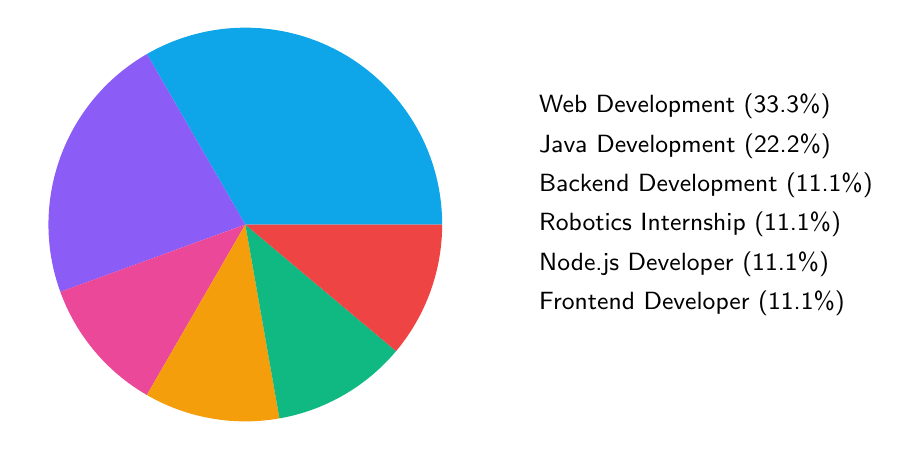
\begin{tikzpicture}
        \coordinate (center) at (0,0);
        \def\radius{2.5cm}
        \pgfmathsetmacro{\totaldata}{3+2+1+1+1+1} % Sum of all data points (3+2+1+1+1+1 = 9)
        
        % Data: Web Development (3), Java Development (2), Backend Development (1), Robotics Internship (1), Node.js Developer (1), Frontend Developer (1)
        % Percentages: 3/9=33.3%, 2/9=22.2%, 1/9=11.1%, 1/9=11.1%, 1/9=11.1%, 1/9=11.1%
        
        \pgfmathsetmacro{\angleA}{3/(\totaldata)*360} % Web Development
        \pgfmathsetmacro{\angleB}{2/(\totaldata)*360} % Java Development
        \pgfmathsetmacro{\angleC}{1/(\totaldata)*360} % Backend Development
        \pgfmathsetmacro{\angleD}{1/(\totaldata)*360} % Robotics Internship
        \pgfmathsetmacro{\angleE}{1/(\totaldata)*360} % Node.js Developer
        \pgfmathsetmacro{\angleF}{1/(\totaldata)*360} % Frontend Developer

        \fill[chart1] (center) -- (0:\radius) arc (0:\angleA:\radius) -- cycle;
        \fill[chart2] (center) -- (\angleA:\radius) arc (\angleA:\angleA+\angleB:\radius) -- cycle;
        \fill[chart3] (center) -- (\angleA+\angleB:\radius) arc (\angleA+\angleB:\angleA+\angleB+\angleC:\radius) -- cycle;
        \fill[chart4] (center) -- (\angleA+\angleB+\angleC:\radius) arc (\angleA+\angleB+\angleC:\angleA+\angleB+\angleC+\angleD:\radius) -- cycle;
        \fill[chart5] (center) -- (\angleA+\angleB+\angleC+\angleD:\radius) arc (\angleA+\angleB+\angleC+\angleD:\angleA+\angleB+\angleC+\angleD+\angleE:\radius) -- cycle;
        \fill[chart6] (center) -- (\angleA+\angleB+\angleC+\angleD+\angleE:\radius) arc (\angleA+\angleB+\angleC+\angleD+\angleE:\angleA+\angleB+\angleC+\angleD+\angleE+\angleF:\radius) -- cycle;

        \node[anchor=west, font=\small] at (3.5, 1.5) {\textcolor{chart1}{$\blacksquare$} Web Development (33.3\%)};
        \node[anchor=west, font=\small] at (3.5, 1) {\textcolor{chart2}{$\blacksquare$} Java Development (22.2\%)};
        \node[anchor=west, font=\small] at (3.5, 0.5) {\textcolor{chart3}{$\blacksquare$} Backend Development (11.1\%)};
        \node[anchor=west, font=\small] at (3.5, 0) {\textcolor{chart4}{$\blacksquare$} Robotics Internship (11.1\%)};
        \node[anchor=west, font=\small] at (3.5, -0.5) {\textcolor{chart5}{$\blacksquare$} Node.js Developer (11.1\%)};
        \node[anchor=west, font=\small] at (3.5, -1) {\textcolor{chart6}{$\blacksquare$} Frontend Developer (11.1\%)};
        \end{tikzpicture}
    \end{center}
\end{card}

\vspace{0.5cm}

\begin{card}
    \subsection*{\textcolor{accent}{Student Internship Details Summary}}
    \vspace{0.3cm}
    \begin{longtable}{@{}p{0.15\textwidth}p{0.15\textwidth}p{0.2\textwidth}p{0.25\textwidth}p{0.2\textwidth}@{}}
        \toprule
        \textbf{Student Name} & \textbf{Student ID} & \textbf{Company} & \textbf{Internship Topic} & \textbf{Duration} \\
        \midrule
        \endhead
        Md Shafaullah & 2054014 12620002031 & Intugine Technologies Pvt. Ltd. & Backend Development using Node.js & 11th July 2022 - 30th June 2023 \\
        Pemba Dorgey Bhutia & 2054015 12620002035 & Oasis Infobyte & WEB DEVELOPMENT AND DESIGNING & 1 Month \\
        Piyush Priyadarshi & 2054016 12620002036 & UPSKILL & Data Science And Machine Learning & 15th JUNE 2023 to 30th JULY 2023 \\
        Satya Prakash & 2054017 12620002048 & UPSKILL & Data Science And Machine Learning & 15th JUNE 2023 to 30th JULY 2023 \\
        Abhay Kumar & 2054018 12620002001 & Internshala & Machine Learning & 6 Weeks \\
        Aditya Kumar & 2054019 12620002003 & EUPHORIA GENX & Android Development of a Note making Application, Chatting Application & 05-06-2023 to 30-07-2023 \\
        Ashish Prasad & 2054020 12620002016 & Octanet & Web Development Internship & 1st July, 2023 - 1st September 2023 \\
        Namrata Sarkar & 2054021 12620002033 & UPSKILL & PYHTON & 15th JUNE 2023 to 30th JULY 2023 \\
        \bottomrule
    \end{longtable}
\end{card}

\vspace{0.5cm}

\begin{card}
    \subsection*{\textcolor{accent}{Summary of Challenges Faced and Solutions}}
    \vspace{0.3cm}
    \begin{longtable}{@{}p{0.05\textwidth}p{0.1\textwidth}p{0.15\textwidth}p{0.2\textwidth}p{0.25\textwidth}p{0.15\textwidth}@{}}
        \toprule
        \textbf{Sl. No.} & \textbf{Class Roll No.} & \textbf{Student Name} & \textbf{Internship/ Training Provider} & \textbf{Internship/ Training Topic Name} & \textbf{Internship/ Training Duration} \\
        \midrule
        \endhead
        24 & 1754029 & Himanshu Tiwari & Internshala & Web Development & 6 Weeks \\
        25 & 1754030 & Aayush Agarwal & Hyland Software Solutions India LLP (Hyland India) (Internship) & Software Development Intern & 11th May, 2020 to 17th July, 2020 \\
        26 & 1754032 & Shubham Kumar Patwarika & DealboX Digisol LLP (Internship) & Room DB Integration and Client Data Entry App Development & 4th May, 2020 to 5th June, 2020 \\
        27 & 1754034 & Ankit Kumar & Internshala & Machine Learning & 27th April, 2020 to 8th June, 2020 (6 Weeks) \\
        28 & 1754035 & Ravi Roshan & Internshala & Web Development & 29th April, 2020 to 24th June, 2020 (8 Weeks) \\
        29 & 1754037 & Aman Bhardwaj & Internshala & Data Science & 28th April, 2020 to 9th June, 2020 (6 Weeks) \\
        30 & 1754038 & Sunny Kumar & JPMORGAN CHASE \& CO. & Software Engineering Virtual Experience (Establishing Financial Data Feeds, Frontend Web Development, Data Visualization with Perspective) & May, 2020 \\
        31 & 1754040 & Ankita Patra & Internshala & Android App Development & 1st May, 2020 to 12th June, 2020 (6 Weeks) \\
        32 & 1754041 & Sania Ajaz & Internshala & Machine Learning with Python & 27th April, 2020 to 8th June, 2020 (6 Weeks) \\
        33 & 1754042 & Mohit Kumar Singh & Internshala & Data Science & 28th April, 2020 to 9th June, 2020 (6 Weeks) \\
        \bottomrule
    \end{longtable}
\end{card}

\clearpage

% ==================== SECTION: RECOMMENDATIONS AND FUTURE OUTLOOK ====================
\section*{\textcolor{accent}{Recommendations and Future Outlook}}
\addcontentsline{toc}{section}{Recommendations and Future Outlook}
{\large\textcolor{muted}{Strategic recommendations for enhancing future internship programs.}}

\vspace{0.5cm}

\begin{card}
    \subsection*{\textcolor{accent}{Recommendations for Future Internships}}
    \vspace{0.3cm}
    To enhance the internship program for future students, a critical review of internship durations and types of engagement is recommended. While a significant number of students undertook shorter programs, such as the numerous 6-week and 8-week internships facilitated by Internshala across various domains like Web Development, Machine Learning, and Data Science, longer durations appear to correlate with more specialized roles. For instance, Darzee offered a 6-month Full Stack Developer role, Intugine Technologies provided a nearly year-long Backend Development opportunity, and Bytelearn and Revirt Space offered 5-month and 4-month SDE Internships, respectively. Future program improvements should encourage students to pursue these extended engagements, which likely offer deeper immersion and more substantial project contributions. Furthermore, the program should continue to support the diverse range of technical topics observed, including Backend, Frontend, Node.js, Java, Python, AI, Machine Learning, Data Analytics, Ethical Hacking, and Cyber Security, ensuring a broad skill development pathway. The inclusion of structured programs, such as the AICTE OIB-SIP internship in Java Development, also presents a valuable model for future offerings.

    Collaboration with industry partners can be significantly enhanced by focusing on the quality and duration of placements. The current report highlights a wide array of partners, from startups like InnoByte Services and Snackbae to established corporations such as Larsen \& Toubro (L\&T), Indian Oil Corporation Limited, Tata Steel Limited, and global entities like JPMORGAN CHASE \& CO. and Accenture Nordic. To deepen these relationships, the department should actively seek to formalize partnerships that facilitate longer-term internships, similar to the 6-month engagement with Darzee or the nearly year-long stint at Intugine Technologies. These extended periods allow for more meaningful project involvement and foster stronger ties between the academic institution and industry. Additionally, exploring and expanding opportunities for virtual experience programs, as offered by JPMORGAN CHASE \& CO. and Accenture Nordic, can broaden access to a wider range of companies and specialized roles, complementing traditional in-person placements.

    For students preparing for future internships, the current experiences underscore the importance of developing robust technical skills in high-demand areas. The prevalence of roles in Web Development (including Full Stack, Frontend, Backend, Node.js, and ReactJS), Machine Learning, Data Science, AI, Java Development, and Python indicates these are critical competencies. Students should prioritize hands-on project work in these domains to build a strong portfolio. Furthermore, based on the varied durations observed, students are advised to actively seek internships that extend beyond the typical 6-8 week period, aiming for opportunities of two months or more. Longer engagements, such as the 4-5 month roles at Bytelearn and Revirt Space, or the 6-month position at Darzee, provide more comprehensive learning and practical application of skills. Finally, students should diversify their search strategies, exploring opportunities not only through online platforms but also directly with companies, academic institutions like IIT Roorkee, and through structured programs like AICTE OIB-SIP, to maximize their exposure to diverse industry environments and challenges.
\end{card}

\vspace{0.5cm}

\begin{card}
    \subsection*{\textcolor{accent}{Top Internship Providers}}
    \vspace{0.3cm}
    \begin{center}
        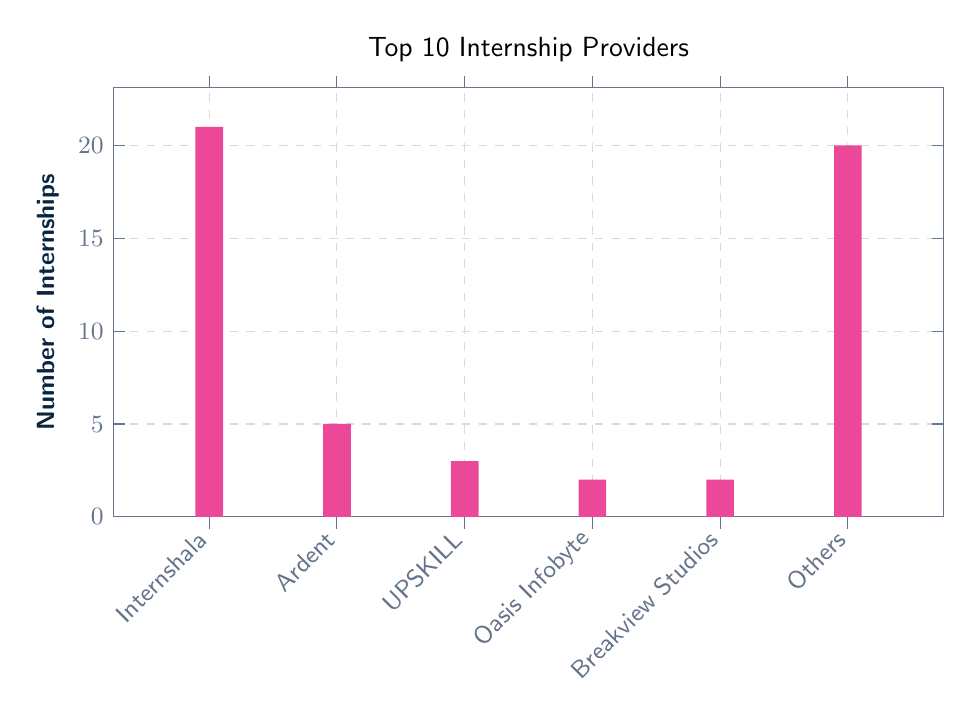
\begin{tikzpicture}
        \begin{axis}[
            institutional bar,
            title={Top 10 Internship Providers},
            x tick label style={rotate=45, anchor=east},
            symbolic x coords={Internshala,Ardent,UPSKILL,Oasis Infobyte,Breakview Studios,Others},
            xtick=data,
            ylabel={Number of Internships},
            ymin=0,
            bar width=10pt,
            legend pos=north west,
            legend style={at={(0.5,-0.2)},anchor=north,legend columns=3},
            width=\textwidth, % Use full minipage width
            height=200pt,
        ]
        \addplot[fill=chart3, draw=none] coordinates {
            (Internshala,21) (Ardent,5) (UPSKILL,3) (Oasis Infobyte,2) (Breakview Studios,2) (Others,20)
        };
        \end{axis}
        \end{tikzpicture}
    \end{center}
\end{card}

\vspace{0.5cm}

\begin{card}
    \subsection*{\textcolor{accent}{Recommendations Matrix for Program Improvement}}
    \vspace{0.3cm}
    \begin{longtable}{@{}p{0.15\textwidth}p{0.2\textwidth}p{0.15\textwidth}p{0.15\textwidth}p{0.15\textwidth}p{0.08\textwidth}p{0.07\textwidth}@{}}
        \toprule
        \textbf{Company Name} & \textbf{Internship/Training Topic} & \textbf{Duration} & \textbf{Student Name} & \textbf{Student ID} & \textbf{Roll Number} & \textbf{Semester} \\
        \midrule
        \endhead
        Ardent Computech Pvt. Ltd. & Ethical Hacking and Cyber Security & 5th June, 2024 - 5th July, 2024 & Dipayan Porel & 2154084 & 12622002067 & 7th \\
        Salahkaar Consultants & Web Applications using React and Django & 10th July, 2024 - 10th October, 2024 & Suraj Roy & 2154085 & 12622002074 & 7th \\
        Internship Studio & Machine Learning & 15th June, 2024 - 20th July,2024 & Debjit Chakraborty & 2154086 & 12622002066 & 7th \\
        Ardent Computech Pvt. Ltd. & Full Stack Development Using Spring Core Spring Boot Hibernate & 6th June, 2024 - 6th July, 2024 & Samrat Ghorui & 2154087 & 12622002072 & 7th \\
        BCGX & Data Science & 19th July, 2024 - 18th August, 2024 & Harsh Sharma & 2154088 & 12622002069 & 7th \\
        AlgoSmiths Softcom & NextJS Developer Internship & 10th July, 2024 - 10th October, 2024 & Bidisa Patra & 2154089 & 12622002065 & 7th \\
        Ardent Computech Pvt. Ltd. & Ethical Hacking and Cyber Security & 5th June, 2024 - 5th July, 2024 & Govind Kumar & 2154090 & 12622002068 & 7th \\
        \bottomrule
    \end{longtable}
\end{card}

\end{document}